
\section{Results}\label{sec:results}

\subsection{Cause--effect pairs}\label{sec:pairs}

Figure~\ref{fig:pairs} and Table~\ref{tab:pairs} give the forced-choice accuracy of the
learned model PDM, LOCI, a Gaussian-process ANM and the four rules on the pair sets. RECI has
the highest accuracy on both chamber sets: $97.9\%$ on the i.i.d.\ pairs and $94.3\%$ on the pairs of
the further recordings. The differences from IGCI ($93.6\%$, $88.5\%$; exact McNemar $p=0.29$ and
$0.17$) are not significant, nor is the difference from PDM on the i.i.d.\ pairs ($p=0.18$); RECI is
significantly more accurate than LOCI ($76.6\%$, $68.0\%$), the Gaussian-process ANM, ANM-HSIC and the
pairwise LiNGAM rule ($p<0.001$ in both sets). On Tübingen LOCI has the highest unweighted accuracy ($64.7\%$, interval
$[54.6,73.9]$, weighted $63.9\%$) and RECI, ANM-HSIC and the LiNGAM rule have $60.8\%$
($[50.6,70.3]$; RECI weighted $70.9\%$, the highest weighted accuracy, with LOCI third). None of these
differences is significant (exact McNemar $p\ge0.23$ for RECI against every other method except PDM).
Our LOCI run uses at most $1000$ rows per pair and the authors' default settings, and its accuracy
may be below published values (Section~\ref{sec:loci-check}). The
Gaussian-process ANM has $55.4\%$ when its $23$ exact ties (a score of zero) are counted as half correct. On the $17$ Sachs pairs (which share $11$ variables) every method lies between $47\%$ and
$65\%$ and every interval contains $50\%$ and is about $50$ points wide. PDM, which reaches $95\%$ on its
held-out simulated test set and $83\%$ on nine unseen simulated families, has $40.2\%$ on Tübingen
(interval $[30.6,50.4]$, exact binomial $p=0.059$ against $50\%$), significantly below RECI (McNemar
$p=0.002$), and is below RECI and IGCI on both chamber sets. The only pair set on which it is
best is the simulated one, which is its own prior.

\begin{figure}[t]
\centering
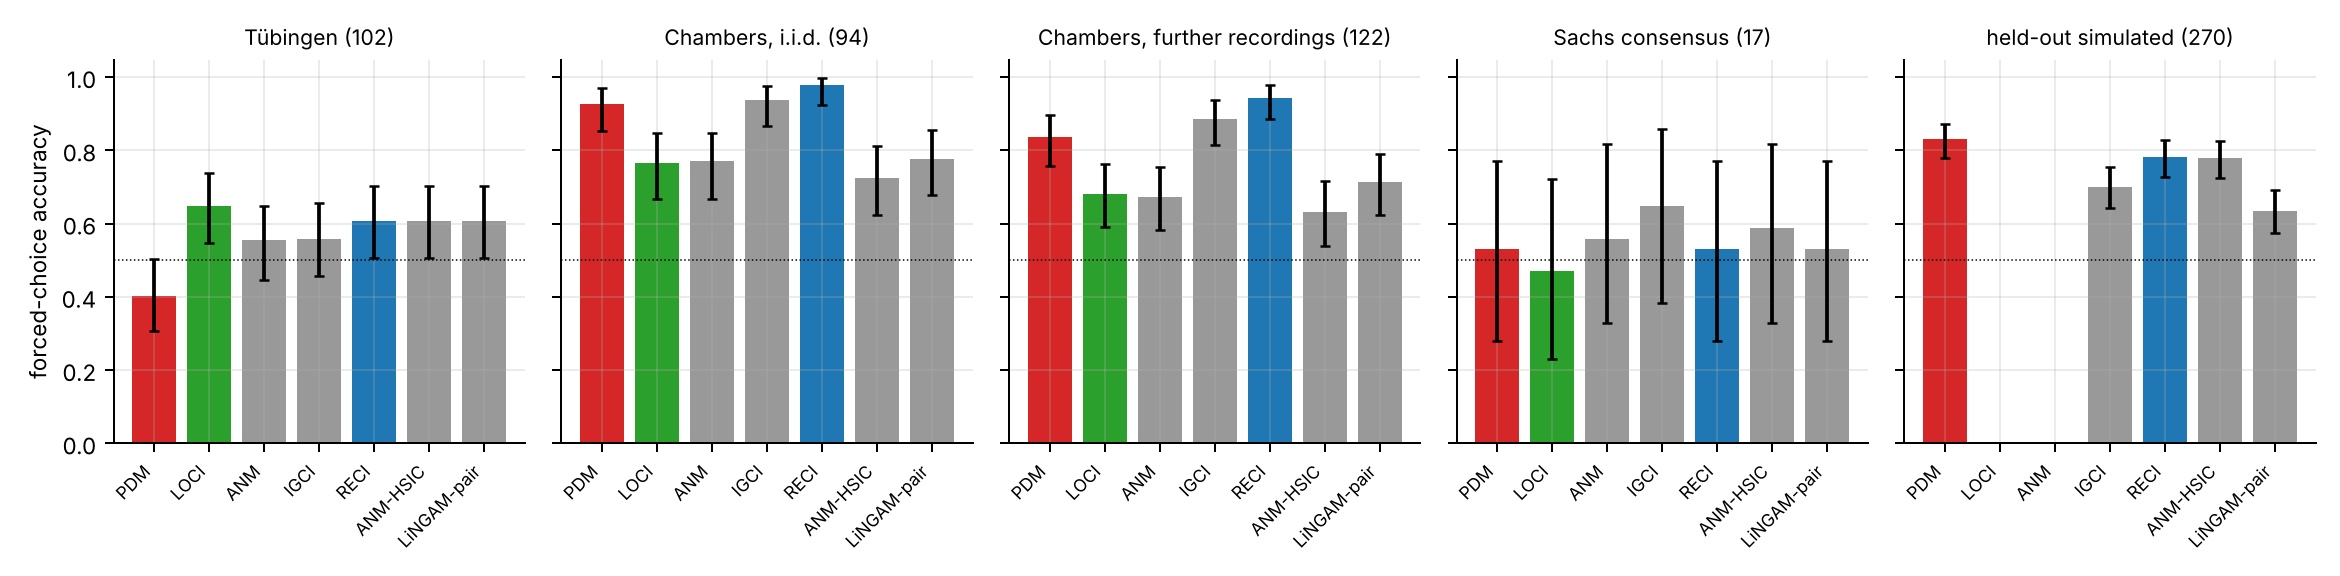
\includegraphics[width=\linewidth]{pairs_accuracy.png}
\caption{Forced-choice accuracy with Clopper--Pearson intervals on five pair sets (pairs or
pair-runs in parentheses). Red: PDM; green: LOCI; blue: RECI; grey: the other rules. Dotted:
chance. LOCI and the Gaussian-process ANM were not run on the simulated families.}
\label{fig:pairs}
\end{figure}

\begin{table}[t]
\caption{Forced-choice accuracy (unweighted; weighted by the official weights for Tübingen).
LOCI and ANM were not run on the simulated families. $^{\dagger}$Exact ties (a score of zero; $23$
pairs) are counted as half correct.}
\label{tab:pairs}
\small
\setlength{\tabcolsep}{2.5pt}
\begin{tabular}{@{}lccccc@{}}
\toprule
Method & Tübingen & chambers iid & chambers, further & Sachs & simulated\\
 & ($102$) & ($94$) & ($122$) & ($17$) & ($270$)\\
\midrule
PDM & 0.402 (0.511) & 0.926 & 0.836 & 0.529 & 0.830\\
LOCI & 0.647 (0.639) & 0.766 & 0.680 & 0.471 & --\\
ANM, Gaussian process$^{\dagger}$ & 0.554 (0.594) & 0.771 & 0.672 & 0.559 & --\\
IGCI & 0.559 (0.664) & 0.936 & 0.885 & 0.647 & 0.700\\
RECI & 0.608 (0.709) & 0.979 & 0.943 & 0.529 & 0.781\\
ANM-HSIC & 0.608 (0.609) & 0.723 & 0.631 & 0.588 & 0.778\\
pairwise LiNGAM & 0.608 (0.620) & 0.777 & 0.713 & 0.529 & 0.633\\
\bottomrule
\end{tabular}
\end{table}

\paragraph{LOCI with more rows.}\label{sec:loci-check} Raising the row cap from $1000$ to $2000$ (the preprocessing of the other
methods) gives $65.7\%$ on Tübingen (interval $[55.6,74.8]$, weighted $66.4\%$) and $97\%$ of the directions agree
with the $1000$-row run, so the cap does not explain the accuracy. We did not reproduce a higher published value
and cannot rule out that the settings or the preprocessing differ from the authors'.

\paragraph{Abstention.} The direction certificate commits on $12$ of the $80$ scorable
Tübingen pairs and is right on $11$. Ranked by its own confidence, RECI is right on $11$ of
its $12$ most confident pairs, and on $21$ of $23$ against $19$ of $23$ at the coverage of the
constant-scale class. On the chamber pairs the certificate is right on all $31$ pairs it
commits to ($94$ pair-runs), as are the RECI and IGCI rankings at that coverage; on the
simulated pairs it is right on $78$ of $83$ against $82$ of $83$ for RECI. At matched coverage the
certificate is therefore not more accurate than RECI; what it adds is that it chooses its
own coverage from the data. The Tübingen result of the certificate is stable over random
draws of the preprocessing ($9/9$, $11/11$, $10/10$ for three further seeds), and its one
error occurred on a pair with $254$ rows.

\subsection{Graphs}\label{sec:graphs}

Table~\ref{tab:graphs} and Figure~\ref{fig:graphs} give the skeleton score on the graph
benchmarks. The ranking of methods depends on the data family.

\begin{table}[t]
\caption{Skeleton precision / recall / $F_1$ against the reference graph (strict); mean over
recordings or subsamples. Sachs: one data set, $17$ reference edges. Chambers i.i.d.: two
recordings, ten subsamples of $4000$ rows each. Chambers with an effective sample size above
$1000$ (two recordings) and below $20$ (seventeen recordings): the first $4000$ rows in time
order. Best $F_1$ in bold.}
\label{tab:graphs}
\scriptsize
\setlength{\tabcolsep}{2pt}
\begin{tabular}{@{}lcccc@{}}
\toprule
Method & Sachs & Chambers iid & ESS $>1000$ & ESS $<20$\\
\midrule
PC, $\alpha=0.05$ & 1.00/0.41/0.58 & 0.40/0.38/0.37 & 0.48/0.28/0.35 & 0.36/0.39/0.37\\
GES-BIC & 1.00/0.41/0.58 & 0.45/0.64/0.49 & 0.74/0.67/\textbf{0.70} & 0.26/0.71/0.38\\
DirectLiNGAM & 1.00/0.35/0.52 & 0.55/0.60/\textbf{0.55} & 0.71/0.63/0.66 & 0.26/0.63/0.37\\
NOTEARS & 1.00/0.18/0.30 & 0.41/0.21/0.27 & 0.33/0.24/0.26 & 0.26/0.45/0.33\\
DAGMA & 1.00/0.29/0.45 & 0.44/0.33/0.36 & 0.44/0.41/0.39 & 0.25/0.52/0.34\\
PCMCI+ & 1.00/0.35/0.52 & 0.39/0.33/0.34 & 0.53/0.29/0.37 & 0.27/0.17/0.20\\
PC, nonparam.\ test & 0.89/0.47/0.62 & 0.38/0.33/0.34 & 0.54/0.34/0.41 & 0.35/0.54/\textbf{0.42}\\
BTAD & 0.89/0.47/0.62 & 0.56/0.36/0.41 & 0.82/0.46/0.58 & 0.60/0.16/0.25\\
LRG & 0.90/0.53/\textbf{0.67} & 0.39/0.48/0.43 & 0.52/0.55/0.53 & 0.51/0.28/0.36\\
CERT-CD, nonparametric & 1.00/0.29/0.45 & 0.29/0.16/0.20 & 0.60/0.18/0.28 & 0.24/0.87/0.37\\
\bottomrule
\end{tabular}
\end{table}

\begin{figure}[t]
\centering
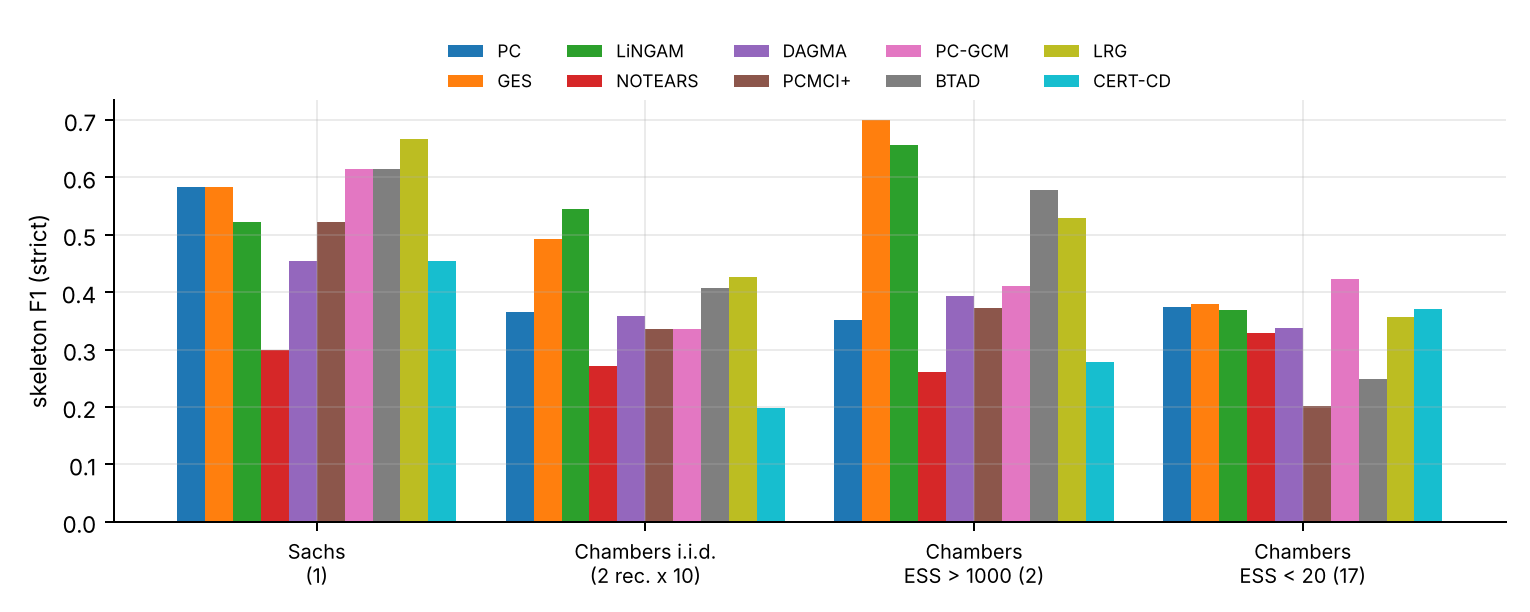
\includegraphics[width=0.95\linewidth]{graph_f1.png}
\caption{Strict skeleton $F_1$ by data family and method.}
\label{fig:graphs}
\end{figure}

\paragraph{Sachs.} The methods we developed that use nonparametric components have the
highest $F_1$ (LRG $0.67$, PC with the nonparametric test $0.62$--$0.64$, BTAD $0.62$), against $0.58$
for PC and GES, $0.52$ for DirectLiNGAM and PCMCI+, $0.45$ for DAGMA and $0.30$ for the linear NOTEARS. The reference network
has $17$ edges, so one edge changes recall by $0.06$ and the differences are not statistically
distinguishable; the classical methods have the highest precision ($1.00$) and the new ones
find a few more edges.

\paragraph{Chambers with independent rows.} DirectLiNGAM and GES have the highest $F_1$. On the two
recordings with i.i.d.\ actuators DirectLiNGAM has $F_1=0.55$ and GES $0.49$, against
$0.32$ to $0.43$ for PC with either test, BTAD and LRG; on the two further recordings with
a large effective sample size GES has $0.70$ and DirectLiNGAM $0.66$. The actuators there
are uniform and the mechanisms may be nearly additive, which would suit DirectLiNGAM (we did not test
this explanation); each group has two recordings and no interval can be given. BTAD has the highest
precision ($0.56$, against $0.55$ for DirectLiNGAM, and $0.82$) at lower recall. The sequential
certificate has the lowest $F_1$ on the i.i.d.\ recordings ($0.20$).

\paragraph{Random-walk recordings.} On the seventeen recordings with an effective sample size
below $20$ every method has a strict $F_1$ between $0.20$ and $0.42$; the best, PC with the nonparametric test,
has precision $0.35$. BTAD has the highest precision ($0.60$, with $2.5$ false edges per
recording against $16$ to $52$ for PC, GES and DirectLiNGAM) and recall $0.16$. PCMCI+, the method
built for autocorrelated series, has recall $0.17$ and $F_1=0.20$ there, as expected when the
recordings contain no usable lag structure (Section~\ref{sec:serial}); DAGMA has $F_1=0.34$. Paired Wilcoxon tests over the $15$
wind-tunnel recordings, with Holm correction over the eleven comparisons, show that BTAD's $F_1$ is
lower than that of ten of the other methods (adjusted $p\le0.02$) and higher than that of PCMCI+; LRG is not
distinguishable from PC, GES or DirectLiNGAM.

\subsection{The walk recordings carry a few independent observations}\label{sec:serial}

Figure~\ref{fig:serial} shows why the walk recordings defeat every method. In the fifteen
wind-tunnel walks the mean lag-1 autocorrelation of the exogenous variables is $0.998$ and
the implied effective sample size is about $3$ of $4000$ rows (range $1.3$ to $12.5$). The mean
cross-correlation between a load and the rotation speed it drives varies by only $0.012$ for lags from $-6$
to $+6$ ($0.974$ to $0.985$), so the recordings also contain no usable lag structure. An i.i.d.\ test
of the independences implied by the graph rejects $40.8$ non-adjacent pairs per recording on the wind-tunnel
walks and a test on $40$ contiguous blocks rejects $8.5$, a ratio of $4.8$; over the seventeen recordings with an
effective sample size below $20$ the ratio is $4.1$ ($38.9$ against $9.5$), over all nineteen $3.7$, for
the pressure-control recording $2$ and for the light-tunnel walk $1$ ($21$ against $21$). The block
test has lower power by construction, so a smaller number of rejections does not by itself show that the
i.i.d.\ rejections are artefacts; it does show that a reference set built with the i.i.d.\ test has
many more pairs than one built with a test that respects serial dependence, and that scores adjusted
for it should be read with caution. Two
recordings of the new set (\texttt{actuators\_white}, \texttt{smooth\_polarizers}) have an
effective sample size above $1000$, and on these two the classical methods have the highest $F_1$; two
recordings are too few to separate effective sample size from device. We did not run a controlled test
(thinning, or a time-series-aware test on the same recordings), which would be the direct evidence.

\begin{figure}[t]
\centering
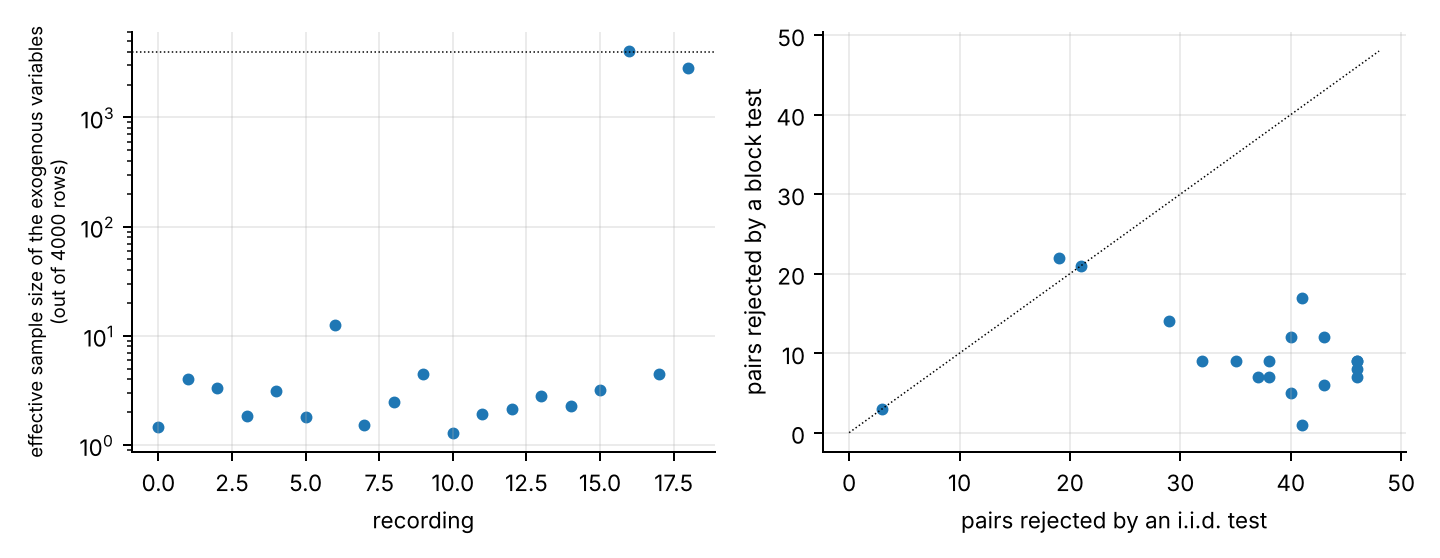
\includegraphics[width=0.9\linewidth]{serial_dependence.png}
\caption{Left: effective sample size (log scale) of the exogenous variables in each of the
nineteen new recordings. Right: number of non-adjacent pairs whose graph-implied independence
is rejected by an i.i.d.\ test and by a block test.}
\label{fig:serial}
\end{figure}

\subsection{Where the new methods help: monitoring and nonlinear mechanisms}\label{sec:monitoring}

On simulated graphs the sequential certificate does what it was designed for
(Table~\ref{tab:monitoring}). When each method is rerun at every sample size from $100$ to
$6400$ on $150$ random eight-node graphs and a graph counts as a failure if any estimate
contains a false edge, CERT-CD fails in $2.7\%$ of the graphs under Laplace errors, against
$27\%$ to $91\%$ for PC, GES and DirectLiNGAM and $39\%$ to $77\%$ for PC with the same
nonparametric test, which is consistent with the delete-on-non-rejection architecture, and not the test, being responsible
(a single comparison). With nonlinear mechanisms the linear test of the certificate fails in $33$
of $60$ graphs under Laplace errors and $28$ of $60$ under Gaussian errors, and the nonparametric
version in $1$ and $2$ of $60$. The guarantee of the linear version is exact only for
Gaussian regression errors, and that of the nonparametric version is asymptotic. The table shows false
edges only, not power: the recall of the nonparametric certificate is $0.00$ at $n=100$ and $0.05$ at
$n=200$ under Laplace errors, and DirectLiNGAM is run on Gaussian errors, which violate its assumption.
These are simulations within the models; on the chambers the false-edge control did not hold
(a false edge adjusted for a reference set built with an i.i.d.\ test in $12$ of $19$ recordings, a strict false edge in $18$, with shuffled rows).

\begin{table}[t]
\caption{Probability that a false edge is ever reported over $n=100,\dots,6400$ ($150$ graphs,
$d=8$), and graphs with a false edge under nonlinear mechanisms ($60$ graphs).}
\label{tab:monitoring}
\small
\begin{tabular}{@{}lcc@{}}
\toprule
Method & Laplace errors & Gaussian errors\\
\midrule
CERT-CD, linear test & 0.027 & 0.040\\
CERT-CD, nonparametric test & 0.060 & 0.047\\
PC, $\alpha=0.05$ / $0.01$ & 0.747 / 0.267 & 0.773 / 0.320\\
PC, nonparametric test, $\alpha=0.05$ / $0.01$ & 0.767 / 0.387 & 0.787 / 0.320\\
GES-BIC & 0.913 & 0.960\\
DirectLiNGAM & 0.760 & 1.000\\
\midrule
nonlinear mechanisms: linear test (of $60$) & 33 & 28\\
nonlinear mechanisms: nonparametric test (of $60$) & 1 & 2\\
\bottomrule
\end{tabular}
\end{table}

\subsection{The gap between simulation and measurement}\label{sec:gap}

The two learned models are accurate on data from their training distribution and lose that
on real data (Table~\ref{tab:gap}). PDM falls from $0.95$ to $0.40$ on Tübingen; LRG falls
from an $F_1$ of $0.86$ on simulated graphs to $0.36$--$0.43$ on the chambers, and its
within-recording ranking of pairs on the wind-tunnel walks is close to chance (mean AUC $0.55$ over $15$
recordings, range $0.51$ to $0.60$).
We cannot say which feature of the real data is responsible; the simulators contain serial
dependence, latent drift, duplicated sensors and several mechanism families and still do not
cover them.

\begin{table}[t]
\caption{Learned models: simulated test against real data.}
\label{tab:gap}
\small
\begin{tabular}{@{}lccc@{}}
\toprule
Model & simulated test & real data & measure\\
\midrule
PDM & 0.95 / 0.83 & 0.40 Tübingen; 0.93, 0.84 chambers & forced accuracy\\
LRG & 0.86 & 0.67 Sachs; 0.43, 0.53, 0.36 chambers & skeleton $F_1$\\
\bottomrule
\end{tabular}
\end{table}
